\chapter{Analytical Development of the Oxygen Transport Model}
\label{ch:o2analytical}

This chapter reduces \cref{eq:ox_cd} to a form that can be solved in closed form, in four steps.
\begin{enumerate}
\item \Cref{sec:ox_scaling} shows by scaling that the concentration is nearly uniform across the gap.
\item \Cref{sec:ox_cup} reduces the problem to an ordinary differential equation for the cup-mixing concentration.
\item \Cref{sec:ox_local} derives the exact relation between the cup-mixing concentration and the concentrations on the floor and the lid.
\item \Cref{sec:ox_imp,sec:ox_mm,sec:ox_pdms} solve the resulting equations for the impermeable, near-anoxic and PDMS/saturated cases.
\end{enumerate}
\Cref{sec:ox_numerical} describes the reduced-order (``1.5-D'') model that solves the same equations without the zero-order simplification, and \cref{sec:ox_choice} states which approximation is suitable where.

\section{Scaling: convection along, diffusion across}
\label{sec:ox_scaling}

Write \cref{eq:ox_cd} in the coordinates of the thin channel, with $x\sim\ell$ (the length over which the width changes), $y\sim w$, $z\sim h$, $u_x\sim\bar U$:
\begin{equation}
\underbrace{u_x\frac{\partial C}{\partial x}}_{\bar U\Delta C/\ell}
=D\Big(\underbrace{\frac{\partial^2C}{\partial x^2}}_{\Delta C/\ell^2}
+\underbrace{\frac{\partial^2C}{\partial y^2}}_{\Delta C/w^2}
+\underbrace{\frac{\partial^2C}{\partial z^2}}_{\Delta C/h^2}\Big).
\label{eq:ox_scaling}
\end{equation}
Relative to diffusion across the gap, axial diffusion is of order $(h/\ell)^2\le10^{-4}$ and transverse diffusion across the width is of order $(h/w)^2\le0.02$, so both are negligible. Convection relative to diffusion across the gap is of order $\Pe_h\,h/\ell$, which near the inlet ($\ell\approx\SI{50}{mm}$) is 0.004 and 0.016 at 0.22 and \SI{1}{\uLmin} and about 2 at \SI{120}{\uLmin}. At the culture flow rates, therefore, the concentration profile across the gap adjusts almost instantly to the local conditions. The axial variation is slow and is controlled by the overall balance between supply and uptake. At \SI{120}{\uLmin} the profile across the gap is still developing over the first few millimetres (\cref{sec:ox_choice}), but there the uptake changes the concentration by only about \SI{1}{\percent}.

\section{Cup-mixing balance and the role of the geometry}
\label{sec:ox_cup}

Define the flow-weighted (cup-mixing) concentration of a cross-section $S(x)$:
\begin{equation}
\Cb(x)=\frac{1}{Q}\iint_{S(x)}u_x\,C\,\dd y\,\dd z .
\end{equation}
Integrate \cref{eq:ox_cd} over the slice between $x$ and $x+\dd x$. Neglect axial diffusion, and let oxygen leave through the floor at the rate $q$ and enter through the lid at the rate $N$ per unit area, with the side walls neglected. Since $Q$ is the same in every section, this gives
\begin{equation}
Q\frac{\dd\Cb}{\dd x}=w(x)\,\big[N(x)-q(x)\big].
\label{eq:ox_cup}
\end{equation}
The geometry enters only through the width multiplying the wall fluxes. Introduce the floor area upstream of $x$,
\begin{equation}
A(x)=\int_0^xw(x')\,\dd x'=w_1L\ln\frac{L}{L-x},
\qquad\frac{\dd A}{\dd x}=w(x),
\label{eq:ox_area}
\end{equation}
so that \cref{eq:ox_cup} becomes
\begin{equation}
Q\frac{\dd\Cb}{\dd A}=N-q .
\label{eq:ox_cupA}
\end{equation}
\Cref{eq:ox_cupA} contains no geometry: per unit area of cell-covered floor, every channel shape behaves the same. The shape matters only through how fast the area accumulates along $x$. In the hyperbolic channel $A(x)$ grows faster than linearly. At $x=\SI{40}{mm}$ the floor upstream is $A=w_1L\ln5=\SI{80.5}{mm^2}$, twice that of a straight channel of width $w_1$. The widening therefore exposes the downstream cells to medium that has already passed over a large upstream area. This is the reason why low shear and low oxygen coincide in this geometry.

\section{Local profile across the gap: exact fully developed solution}
\label{sec:ox_local}

To close \cref{eq:ox_cupA} we need $q$ and $N$, which depend on the wall concentrations $\Cbot$ and $\Ctop$, not on $\Cb$. These are related by the local profile across the gap. In the quasi-equilibrium of \cref{sec:ox_scaling}, $\partial C/\partial x$ is independent of $z$ and equal to $\dd\Cb/\dd x$ (``fully developed'' mass transfer). The leading-order balance in the core of the section is then
\begin{equation}
D\frac{\partial^2C}{\partial z^2}=u_x(z)\frac{\dd\Cb}{\dd x},
\qquad u_x=\frac{6Q}{wh}\,\eta(1-\eta),\quad\eta=\frac zh .
\end{equation}
Substituting $\dd\Cb/\dd x$ from \cref{eq:ox_cup},
\begin{equation}
\frac{\dd^2C}{\dd\eta^2}=\frac{6h}{D}\,(N-q)\,\eta(1-\eta),
\qquad
\left.\frac{\dd C}{\dd\eta}\right|_{\eta=0}=\frac{qh}{D},\quad
\left.\frac{\dd C}{\dd\eta}\right|_{\eta=1}=\frac{Nh}{D},
\label{eq:ox_local_ode}
\end{equation}
where the boundary conditions are \cref{eq:ox_bc_floor,eq:ox_bc_pdms} written for the fluxes $q$ and $N$. Integrating once,
\begin{equation}
\frac{\dd C}{\dd\eta}=\frac hD\Big[q+6(N-q)\Big(\frac{\eta^2}{2}-\frac{\eta^3}{3}\Big)\Big],
\end{equation}
which satisfies the condition at $\eta=1$ automatically, as the overall balance requires. Integrating again from the floor,
\begin{equation}
C(\eta)=\Cbot+\frac hD\Big[q\,\eta+(N-q)\Big(\eta^3-\frac{\eta^4}{2}\Big)\Big].
\label{eq:ox_profile}
\end{equation}
\paragraph{Impermeable lid ($N=0$).} \Cref{eq:ox_profile} reduces to
\begin{equation}
C(\eta)-\Cbot=\frac{qh}{D}\left(\eta-\eta^3+\frac{\eta^4}{2}\right),\qquad
\Ctop-\Cbot=\frac{qh}{2D}.
\label{eq:ox_profile_imp}
\end{equation}
\paragraph{Cup-mixing relations.} Weighting \cref{eq:ox_profile} with $u_x\propto6\eta(1-\eta)$ uses the integrals $\int_0^16\eta(1-\eta)\eta\,\dd\eta=\tfrac12$ and $\int_0^16\eta(1-\eta)(\eta^3-\eta^4/2)\,\dd\eta=\tfrac{9}{70}$. The result is
\begin{equation}
\Cb-\Cbot=\frac hD\left(a_sq-a_cN\right),\qquad
\Ctop-\Cb=\frac hD\left(a_sN-a_cq\right),\qquad
a_s=\frac{13}{35},\ a_c=-\frac{9}{70}.
\label{eq:ox_superpos}
\end{equation}
For a single wall with constant flux and the other wall impermeable, the Sherwood number based on $2h$ is $\Sh=2/a_s=70/13=5.385$. For equal fluxes at both walls it is $2/(a_s+a_c)=140/17=8.235$. These are the classical values for parallel plates \citep{ShahLondon1978}, which confirms the derivation.

\paragraph{How large is the drop across the gap?} With full uptake $q=\qmax$, the floor is lower than the lid by $\qmax h/(2D)$ (IMP) or $\qmax h/D$ (balanced supply through the lid, where the profile is linear). Relative to $\Csat$, these are $\Da_w/2=\SI{0.54}{\percent}$ and $\Da_w=\SI{1.09}{\percent}$ (\cref{fig:o2_z}). Diffusion across the gap is therefore never the bottleneck. The availability of oxygen at the cells is decided by the axial balance \cref{eq:ox_cupA}.

\begin{figure}[htbp]
\centering
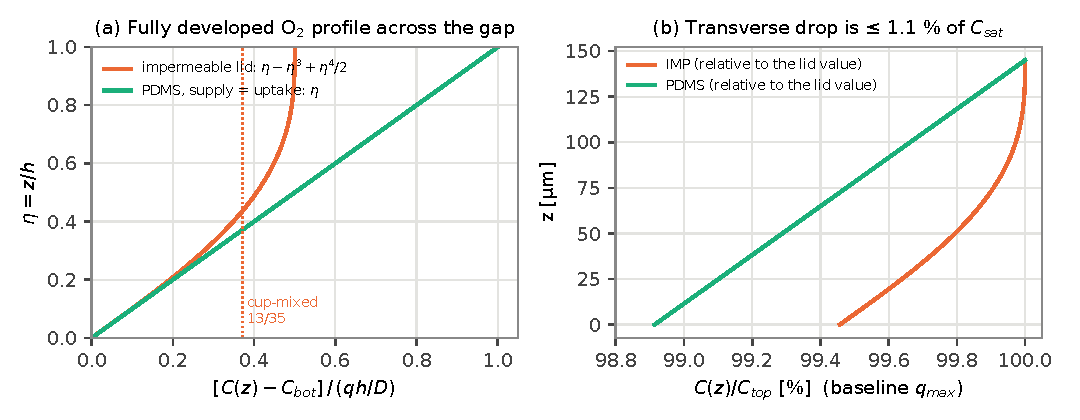
\includegraphics[width=0.95\linewidth]{oxygen_transverse_profile.pdf}
\caption{Fully developed oxygen profile across the gap \tagT. (a) Dimensionless profiles from \cref{eq:ox_profile}: impermeable lid (uptake balanced by axial depletion) and PDMS lid with supply equal to uptake (pure diffusion, linear). The dotted line is the cup-mixing value 13/35 for the impermeable lid. (b) The same profiles for the baseline uptake: the variation across the gap is at most \SI{1.1}{\percent} of the lid value.}
\label{fig:o2_z}
\end{figure}

\section{Solution I: impermeable walls, zero-order uptake}
\label{sec:ox_imp}

With $N=0$ and $q=\qmax$, \cref{eq:ox_cupA} integrates directly with $\Cb(0)=\Csat$:
\begin{equation}
\Cb(x)=\Csat-\frac{\qmax}{Q}A(x)=\Csat-\frac{\qmax w_1L}{Q}\ln\frac{L}{L-x},
\label{eq:ox_imp}
\end{equation}
and from \cref{eq:ox_superpos} the floor concentration is
\begin{equation}
\frac{\Cbot(x)}{\Csat}=1-\Da_{\mathrm{conv}}\frac{A(x)}{A_{\mathrm{cells}}}-\frac{13}{35}\Da_w .
\label{eq:ox_imp_bot}
\end{equation}
The oxygen at the cells decreases linearly with the upstream cell area, and therefore logarithmically with $x$, steepening towards the outlet. The last term is a constant offset of \SI{0.4}{\percent}. If $\Da_{\mathrm{conv}}<1$, the oxygen lost along the whole culture section is the fraction $\Da_{\mathrm{conv}}$ of the inlet supply: \SI{1.3}{\percent} at \SI{120}{\uLmin}. If $\Da_{\mathrm{conv}}>1$, the floor runs out of oxygen at the position where $\Cbot=0$. Neglecting the \SI{0.4}{\percent} offset,
\begin{equation}
x_{\mathrm{crit}}=L\left[1-\exp\!\left(-\frac{Q\Csat}{\qmax w_1L}\right)\right],
\label{eq:ox_xcrit}
\end{equation}
which is \SI{13.9}{mm} at \SI{0.22}{\uLmin} and \SI{38.7}{mm} at \SI{1}{\uLmin} \tagM. The minimum flow rate that keeps the whole culture section supplied by convection alone is
\begin{equation}
Q_{\min}=\frac{\qmax A_{\mathrm{cells}}}{\Csat}=\frac{\qmax w_1L\ln(w_{\max}/w_1)}{\Csat}=\SI{1.55}{\uLmin}.
\label{eq:ox_qmin}
\end{equation}
\Cref{eq:ox_xcrit} contains neither $D$ nor $h$. With impermeable walls the location of anoxia is set entirely by the ratio of convective supply to uptake, and changing the gap or the diffusivity does not move it. Since the shear scales as $\taw\propto Q/h^2$, a taller channel at the same shear requires a larger $Q\propto h^2$ and so delivers more oxygen. This is the coupling exploited in the design discussion of \cref{ch:o2results}.

\section{Solution II: approach to anoxia with Michaelis--Menten kinetics}
\label{sec:ox_mm}

Zero-order uptake stops being valid as $\Cbot\to\Km$. For $\Cbot\ll\Km$ the uptake is first order, $q\approx(\qmax/\Km)\Cbot$. Using $\Cbot=\Cb-a_s(h/D)q$ from \cref{eq:ox_superpos} (with $N=0$), the uptake can be written in terms of the cup-mixing concentration as two resistances in series:
\begin{equation}
q=k_{\mathrm{eff}}\,\Cb,\qquad
\frac{1}{k_{\mathrm{eff}}}=\underbrace{\frac{\Km}{\qmax}}_{\text{uptake}}+\underbrace{\frac{13}{35}\frac hD}_{\text{diffusion across }h}
=\SI{1.58e4}{}+\SI{1.80e4}{}\ \si{s/m}.
\end{equation}
\Cref{eq:ox_cupA} then gives an exponential decay in area beyond the point $A_c=A(x_{\mathrm{crit}})$:
\begin{equation}
\Cb(A)=\Cb(A_c)\exp\!\left[-\frac{k_{\mathrm{eff}}(A-A_c)}{Q}\right],
\qquad
\frac{Q}{k_{\mathrm{eff}}}=\SI{0.12}{mm^2}\ (0.22),\ \SI{0.56}{mm^2}\ (1\ \si{\uLmin}).
\label{eq:ox_mm_tail}
\end{equation}
At the local widths (\SI{1.4}{mm} and \SI{4.4}{mm}), these areas correspond to a decay length of only about \SI{0.1}{mm}. The transition from normoxia to anoxia is therefore sharp. Without the diffusion resistance, the Michaelis--Menten balance $Q\,\dd C/\dd A=-\qmax C/(\Km+C)$ has the implicit exact solution
\begin{equation}
(C-C_0)+\Km\ln\frac{C}{C_0}=-\frac{\qmax}{Q}(A-A_0),
\label{eq:ox_mm_implicit}
\end{equation}
which reduces to \cref{eq:ox_imp} for $C\gg\Km$ and to an exponential for $C\ll\Km$. In practice, $x_{\mathrm{crit}}$ from \cref{eq:ox_xcrit} marks the edge of an anoxic region with a sub-millimetre transition zone.

\section{Solution III: permeable (PDMS) and saturated lid}
\label{sec:ox_pdms}

With the Robin condition $N=\kp(\Csat-\Ctop)$, the lid concentration is eliminated using \cref{eq:ox_superpos}:
\begin{equation}
N=k'\left[(\Csat-\Cb)-\frac{9}{70}\frac hDq\right],\qquad
k'=\frac{\kp}{1+\frac{13}{35}\Bi}=\SI{5.13e-6}{m/s}.
\label{eq:ox_N}
\end{equation}
With zero-order uptake ($q=\qmax$, valid because $C\gg\Km$ throughout, as shown below), \cref{eq:ox_cupA} is a linear first-order equation in $\Cb$:
\begin{equation}
Q\frac{\dd\Cb}{\dd A}=k'\left(\Cb_\infty-\Cb\right),\qquad
\Cb_\infty=\Csat-\frac{\qmax}{k'}-\frac{9}{70}\frac{h\qmax}{D},
\end{equation}
with solution
\begin{equation}
\Cb(x)=\Cb_\infty+(\Csat-\Cb_\infty)\exp\!\left[-\frac{k'A(x)}{Q}\right].
\label{eq:ox_pdms}
\end{equation}
The cup-mixing concentration relaxes exponentially, in terms of the upstream cell area, to an equilibrium in which the lid supplies exactly what the cells consume. In that equilibrium $N=\qmax$, the profile across the gap is linear, and from $\Ctop=\Csat-\qmax/\kp$ and $\Ctop-\Cbot=\qmax h/D$,
\begin{equation}
\frac{C_{\mathrm{bot},\infty}}{\Csat}=1-\frac{1}{\Phi_{\mathrm{PDMS}}}-\Da_w=1-0.040-0.011=0.949 .
\label{eq:ox_pdms_inf}
\end{equation}
This depends neither on $Q$ nor on the geometry. The relaxation area $Q/k'$ converts through \cref{eq:ox_area} into a relaxation length from the inlet, $x^*=L[1-\exp(-Q/(k'w_1L))]$. It is \SI{0.71}{mm} at \SI{0.22}{\uLmin} and \SI{3.1}{mm} at \SI{1}{\uLmin}, so the equilibrium governs almost the whole channel. At \SI{120}{\uLmin}, $Q/k'=\SI{390}{mm^2}$ exceeds the whole cell area, so the lid hardly matters: convection keeps the concentration near $\Csat$.

\paragraph{Saturated lid.} For $\kp\to\infty$, $k'\to D/(a_sh)$, the equilibrium is $C_{\mathrm{bot},\infty}=\Csat(1-\Da_w)=0.989\,\Csat$, and it is reached within $x^*=0.07$, 0.30 and \SI{25.6}{mm} at the three flow rates.

\paragraph{Validity.} With the baseline parameters $\Cbot\ge0.95\,\Csat=268\,\Km$, so the zero-order assumption holds to better than \SI{0.4}{\percent}. The PDMS result requires $\Phi_{\mathrm{PDMS}}>1$. If the lid permeability or thickness were such that $\kp\Csat<\qmax$, the lid alone could not feed the cells, and the IMP-type depletion of \cref{sec:ox_imp} would reappear, delayed in $x$.

\section{Reduced-order numerical model (1.5-D)}
\label{sec:ox_numerical}

The closed forms use zero-order kinetics. The general case, with Michaelis--Menten uptake, any lid condition and any flow rate, is solved by integrating \cref{eq:ox_cup} numerically. At each $x$ the local fluxes are found from three coupled algebraic relations,
\begin{equation}
q=\qmax\frac{\Cbot}{\Km+\Cbot},\qquad
\Cbot=\Cb-\frac hD\left(a_sq-a_cN\right),\qquad
N=k'\left[(\Csat-\Cb)+a_c\frac hDq\right],
\end{equation}
which reduce to one non-linear equation for $q$, solved by bisection (Brent's method). The ODE is integrated with an adaptive Runge--Kutta method (relative tolerance $10^{-8}$) from $\Cb(0)=\Csat$ to $x_t$ (code in \cref{app:repro}). Two checks were made:
\begin{itemize}
\item the integrated uptake equals the oxygen lost by the flow to within \SI{0.03}{\percent} in all nine cases (global mass balance);
\item in the zero-order range the numerical solution reproduces the closed forms \cref{eq:ox_imp,eq:ox_pdms} (\cref{fig:o2_axial}); for example, at $x=\SI{45}{mm}$ and \SI{1}{\uLmin} with a PDMS lid, $\Cbot/\Csat=0.9496$ (numerical) against 0.9494 (closed form).
\end{itemize}

\section{Which approximation is suitable where}
\label{sec:ox_choice}

\begin{table}[htbp]
\centering
\caption{Analytical approximations for oxygen transport in the widening chip and their range of validity.}
\label{tab:ox_models}
\small
\begin{tabularx}{\linewidth}{@{}p{0.27\linewidth}X p{0.2\linewidth}@{}}
\toprule
Approximation & Valid when & Use\\
\midrule
Pure diffusion across the gap (linear profile) & local supply equals uptake ($\dd\Cb/\dd x=0$) & PDMS/SAT equilibrium\\
Fully developed profile, \cref{eq:ox_superpos} & $\Pe_h h/\ell\ll1$; beyond the concentration entrance length & 0.22 and \SI{1}{\uLmin}; all $x$\\
Cup-mixing balance \cref{eq:ox_cupA} & $\Pe_L\gg1$; side walls negligible & all cases\\
Zero-order closed forms (I, III) & $\Cbot\gg\Km$ & before $x_{\mathrm{crit}}$; PDMS/SAT everywhere\\
First-order tail (II) & $\Cbot\ll\Km$ & just beyond $x_{\mathrm{crit}}$\\
Full MM, 1.5-D numerical & all of the above but kinetics general & reference solution\\
3D CFD (UDS) & always & side-wall layers, outlet corner\\
\bottomrule
\end{tabularx}
\end{table}

The concentration entrance length for parallel plates, $L_c\approx0.0115\,\Pe_{2h}\,(2h)$ \citep{ShahLondon1978} with $\Pe_{2h}=\bar U_0\,2h/D$, is 0.008, 0.037 and \SI{4.4}{mm} at the three flow rates. Within it, the concentration boundary layer on the floor is thinner than the gap and $\Cbot$ is closer to $\Cb$ than the fully developed relation predicts. The fully developed model therefore slightly over-predicts the depletion near the inlet at \SI{120}{\uLmin}, by at most $a_s\Da_w=\SI{0.4}{\percent}$ of $\Csat$. This error is conservative and negligible. A Lévêque-type developing-layer analysis is therefore unnecessary. The most suitable model for this geometry is the cup-mixing balance with the exact fully developed closure. It is accurate wherever the lubrication flow is accurate, and it misses only the three-dimensional side-wall and corner effects.
